\documentclass[11pt,a4paper]{article}

% -------------------------------------------------
% Pacchetti
% -------------------------------------------------
\usepackage[margin=2.5cm]{geometry}
\usepackage{amsmath,amssymb}
\usepackage{siunitx}
\usepackage{graphicx}
\usepackage{microtype} % aiuta a ridurre Overfull/Underfull hbox
\usepackage{caption}
\usepackage{subcaption}
\usepackage{hyperref}

% Impostazioni didascalie: niente hbox lunghi
\captionsetup{format=plain,justification=raggedright,singlelinecheck=false}

\title{Hover Disc a 20\,cm: Modello con Cuscino Centrale e Getto di Corona}
\author{}
\date{\today}

\begin{document}
\maketitle

\section{Schema geometrico e notazioni}

\begin{figure}[ht]
  \centering
  % usa \linewidth per evitare overfull dei float larghi
  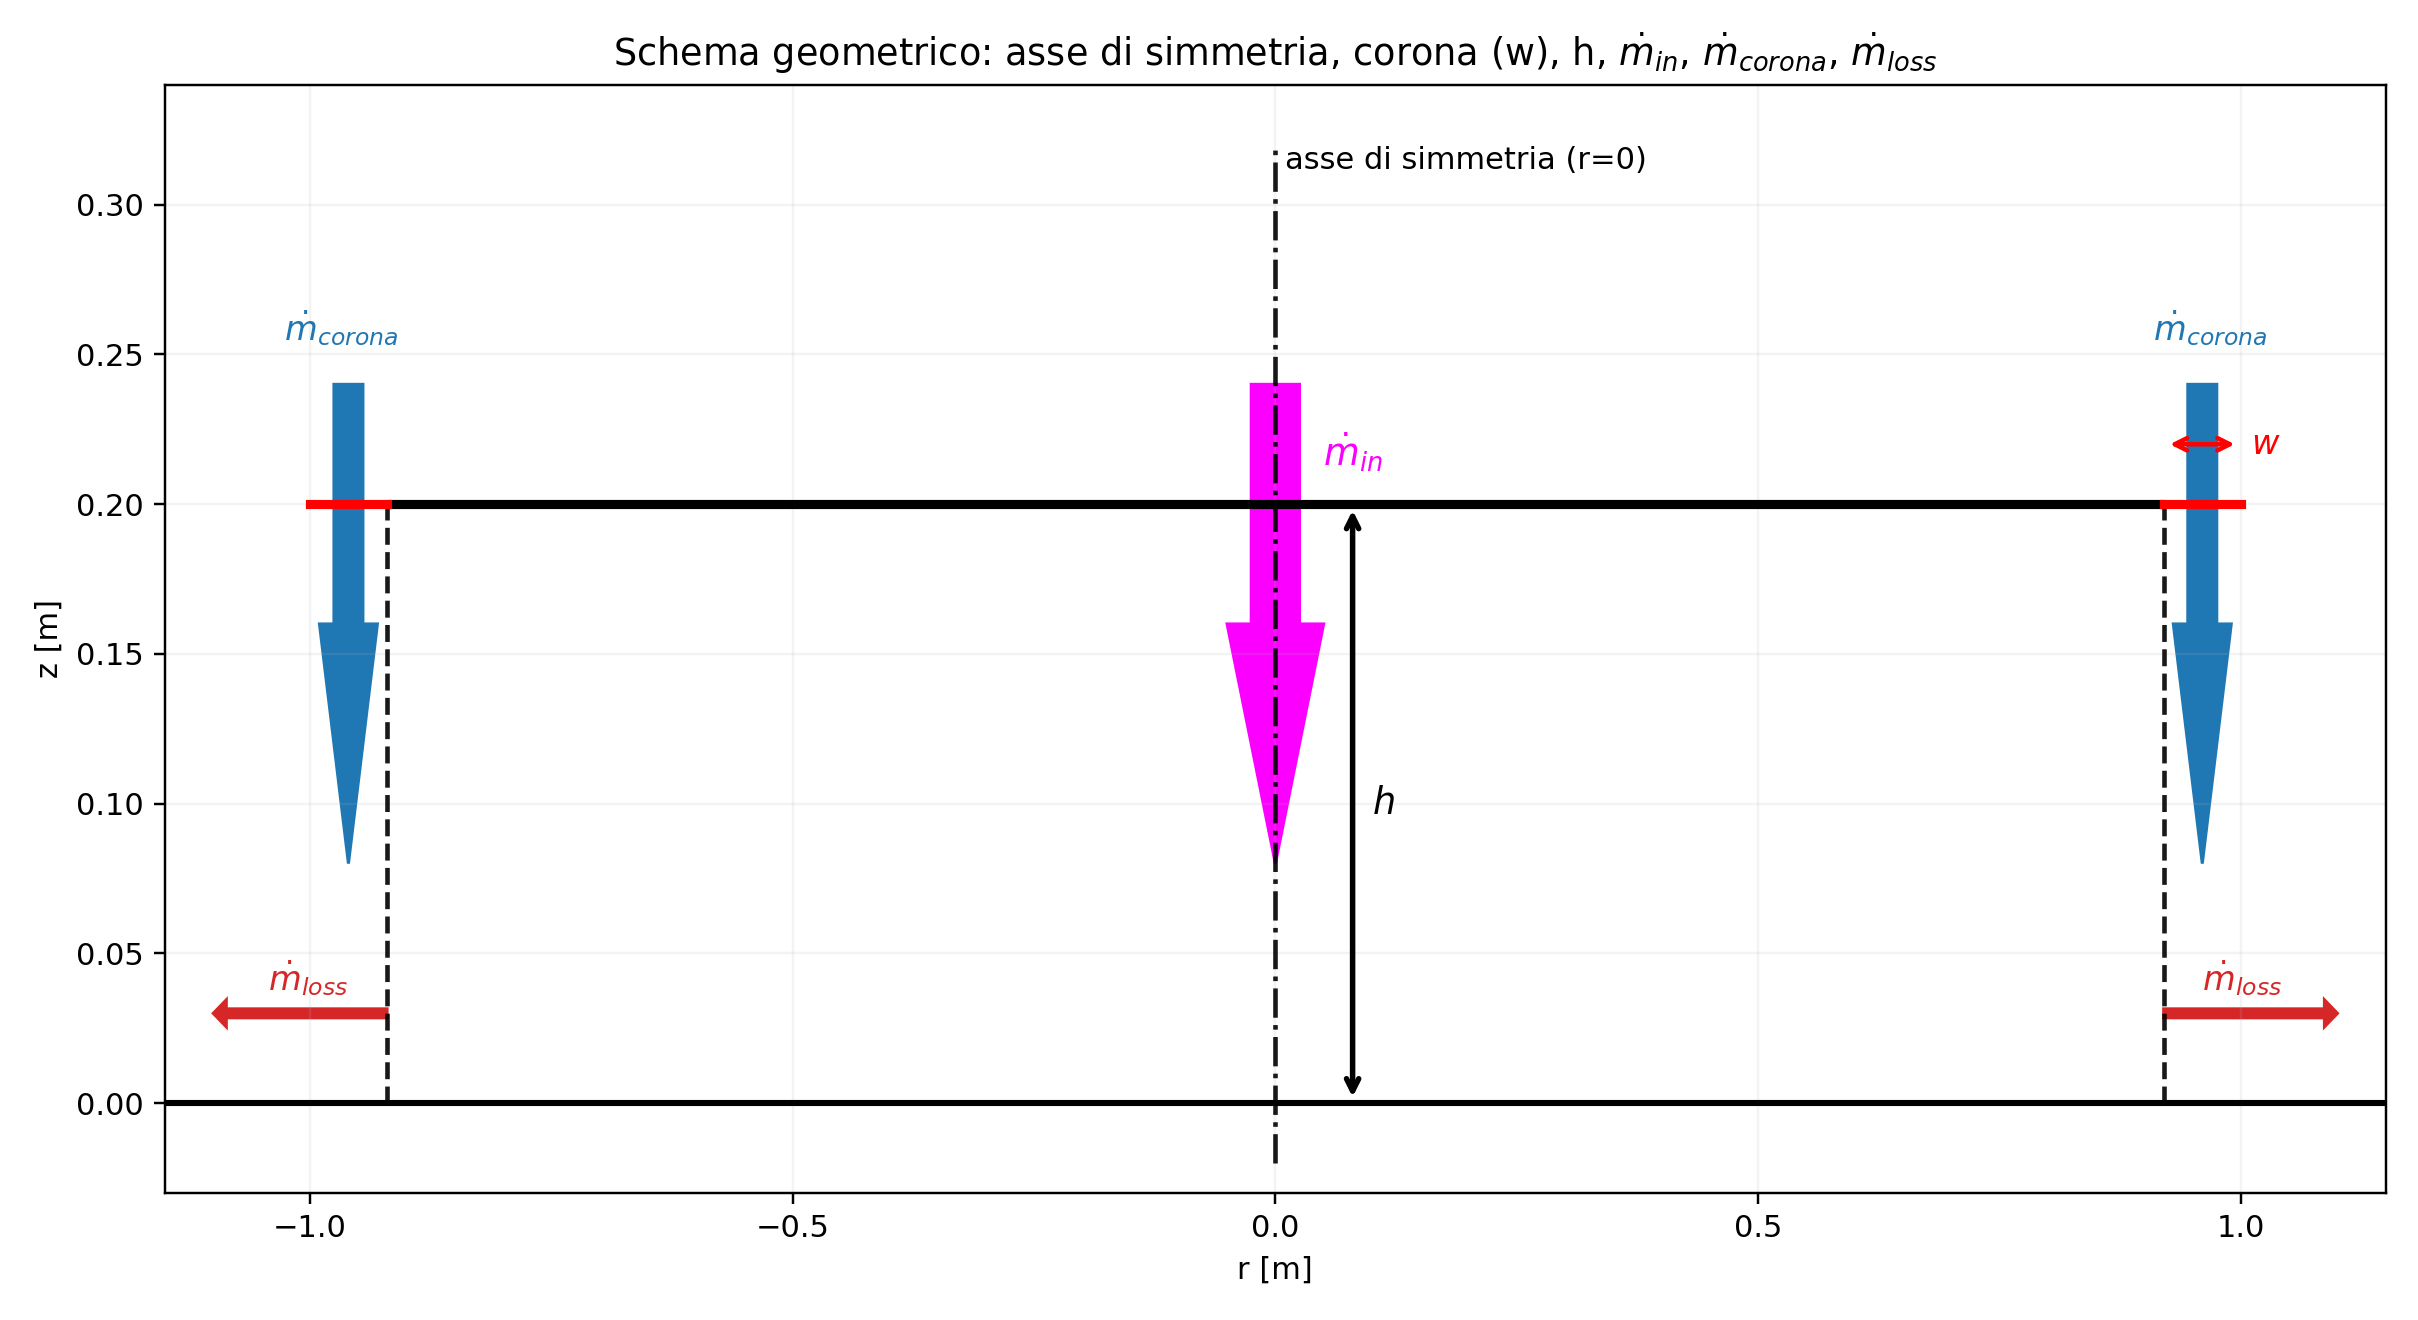
\includegraphics[width=0.8\linewidth]{./figures/schema_geometry.png}
  % Evita math in PDF strings con \texorpdfstring
  \caption{Schema della sezione assiale: disco sospeso a quota \(h\), zona centrale a pressione quasi costante \texorpdfstring{$p_c$}{pc}, fascia di getto periferico di larghezza \texorpdfstring{$w$}{w}, portata entrante \texorpdfstring{$\dot{m}_{\mathrm{in}}$}{mdot\_in}, portata della corona \texorpdfstring{$\dot{m}_{\mathrm{corona}}$}{mdot\_corona} e flusso disperso laterale \texorpdfstring{$\dot{m}_{\mathrm{loss}}$}{mdot\_loss}. L'asse di simmetria a \texorpdfstring{$r=0$}{r=0} è mostrato.}
  \label{fig:schemageo}
\end{figure}

Nel presente modello semplificato non consideriamo pareti laterali rigide né air--curtain: l'unico \emph{sigillo} è costituito dalla corona periferica. Le grandezze in figura sono:
\begin{itemize}
  \item \(R_{\mathrm{tot}}\): raggio totale del disco, pari al raggio esterno della corona;
  \item \(w\): larghezza della corona, tale che il raggio interno del cuscino centrale sia \(R_i = R_{\mathrm{tot}} - w\);
  \item \(h\): altezza del disco rispetto al suolo, ossia distanza della faccia inferiore di contatto del cuscino;
  \item \(\dot{m}_{\mathrm{in}}\): portata massica d'aria che entra nella zona centrale dal getto o dal sistema di alimentazione;
  \item \(\dot{m}_{\mathrm{corona}}\): portata massica che percorre la corona periferica e getta radialmente in uscita;
  \item \(\dot{m}_{\mathrm{loss}}\): portata massica che fuoriesce radialmente dal bordo esterno senza contribuire al cuscino centrale (perdita laterale).
\end{itemize}

\section{Equazioni fondamentali}

\subsection{Pressione portante nel cuscino centrale}
L'area effettiva che genera portanza è quella del disco di raggio \(R_i\); la pressione centrale necessaria a sostenere un carico utile \(m\) è
\begin{equation}
  p_c = \frac{m g}{\pi R_i^2}.
\end{equation}

\subsection{Bilancio di massa nella zona centrale}
Assumendo stazionarietà e che la corona non entri nel flusso del cuscino centrale,
\begin{equation}
  \dot{m}_{\mathrm{in}} = \dot{m}_{\mathrm{loss}}.
\end{equation}
Questo equilibrio garantisce che la pressione rimanga stabile nella regione interna.

\subsection{Portata nella corona periferica}
La corona è modellata come un getto anulare di spessore \(t\) (fessura) a raggio \(R_i\). La portata massica nella corona è
\begin{equation}
  \dot{m}_{\mathrm{corona}} = \rho \, (2\pi R_i\, t)\, V_{\mathrm{jet}},
\end{equation}
dove \(V_{\mathrm{jet}}\) è la velocità del getto nella corona.

\subsection{Perdita laterale al bordo esterno}
Nel punto \(r = R_{\mathrm{tot}}\) l'aria può uscire verso l'ambiente (\(p=0\)). Si adottano due modelli.

\paragraph{Modello orifizio (inerziale).}
Se il flusso è dominato da effetti dinamici,
\begin{equation}
  A_e = 2\pi R_{\mathrm{tot}}\, h, 
  \qquad
  \dot{m}_{\mathrm{loss}} = \rho\, C_d\, A_e \sqrt{\frac{2 p_c}{\rho}}
  = C_d\, (2\pi R_{\mathrm{tot}}\, h)\, \sqrt{2\,\rho\,p_c}.
\end{equation}

\paragraph{Modello di lubrificazione (viscoso).}
Se il flusso è dominato da attrito viscoso in una fuga radiale,
\begin{equation}
  Q_{\mathrm{loss}} = \frac{\pi\, h^3\, p_c}{6\,\mu\, \ln\!\left(\tfrac{R_{\mathrm{tot}}}{R_i}\right)}, 
  \qquad
  \dot{m}_{\mathrm{loss}} = \rho\, Q_{\mathrm{loss}}.
\end{equation}

La scelta fra i due modelli dipende dal numero di Reynolds nel gap \(h\).

\subsection{Potenza ideale minima}
La potenza ideale richiesta per il cuscino è
\begin{equation}
  P_{\mathrm{cuscino}}^{\mathrm{ideal}} = p_c\, Q_{\mathrm{in}} = p_c\, \frac{\dot{m}_{\mathrm{in}}}{\rho}.
\end{equation}
La potenza cinetica del getto nella corona (facoltativa) è
\begin{equation}
  P_{\mathrm{jet}} = \tfrac12 \dot{m}_{\mathrm{corona}}\, V_{\mathrm{jet}}^2.
\end{equation}

\section{Criteri di scelta del modello}
Il criterio pratico per distinguere i due regimi si basa sul numero di Reynolds:
\begin{equation}
  Re = \frac{\rho U h}{\mu}.
\end{equation}
\[
\begin{cases}
Re \gg 2000 & \text{modello orifizio (inerziale)},\\
Re \lesssim 2000 & \text{modello di lubrificazione (viscoso)}.
\end{cases}
\]

\section{Considerazioni e sviluppi}
Sono trascurati gli effetti di compressibilità, l'interazione tra getto di corona e cuscino, le perdite locali e la non planarità del suolo.
Nei prossimi sviluppi si potranno:
\begin{itemize}
  \item implementare simulazioni numeriche per varie configurazioni geometriche;
  \item generare mappe di pressione e velocità coerenti con il modello scelto;
  \item introdurre un air--curtain per ridurre \(\dot{m}_{\mathrm{loss}}\) e migliorare la stabilità.
\end{itemize}

% -------------------------------------------------
% BibTeX: elimina l'avviso "I found no \citation commands"
% (usa il tuo tex/refs.bib esistente)
% -------------------------------------------------
\nocite{*}
\bibliographystyle{plain}
\bibliography{refs}

\end{document}
